
\chapter{Codec}


Die Grundidee der Komprimierung basiert darauf, einen zu kodierenden Pixelwert
$p_{i}$  \"uber ein vorhergehenden (decodierten) Referenzpixel $b_{ref(i,d)}$ anzun\"ahern:

\begin{equation}
    b_i = b_{ref(i,dir)} + c_{val}
\label{form:enc-basic}
\end{equation}

F\"ur die eigentlich Kodierung sind an dieser Stelle nur relevant, welchen Wert
$c_{val}$ und $dir$ annehmen. $dir$ steht in diesem Kontext f\"ur \textit{direction} und
beschreibt mit $ref(i,dir)$ einen Nachbarpixel des Pixel $p_i$ in eine Richtung,
die $dir$ kodiert. Der Ann\"aherungswert $c_{val}$ \textit{change value} wird implizit 
bestimmt. Durch die Abweichung
\begin{equation}
    d = b_i - p_i
\label{form:enc-dist}
\end{equation}
kann unter der Annahme $b_{i+1} \approx b_i$ eine Entscheidung dar\"uber getroffen 
werden, ob $c_{val}$ f\"ur den n\"achsten Schritt erh\"oht oder verringert werden
sollte. Diese Information wird im Folgenden als $c$ verstanden. Eine Variante
$c_{va]}$ zu aktualisieren zeigt Listing~\ref{lst:codec-updt-x}.
%
\begin{lstlisting}[caption=Aktualisierung von $c_{val}$ anhand des $c$-Flags,%
                   label=lst:codec-updt-x]
if (c) {
    c_val = c_val + c_val/2;
} else {
    c_val = -c_val;
    if (abs(c_val)>=CMPR_C_MIN*2) 
        c_val /= 2;
}
\end{lstlisting}
%
Daraus lassen sich  zwei Eigenschaften ableiten. Zum einen muss $c_{val}$ im
laufe der Kodierung mitbestimmt und f\"ur jeweilige Referenzpixel gespeichert werden, aber
zum anderen verringert sich auch die \textit{distance} $d$, wenn tats\"achlich
\"ahnliche Pixelwerte aufeinander folgen, da sich die rekonstruierten Werte
``einschwingen''.
Faktisch muss bei der Enkodierung eines Pixels $p_i$ folgende Gleichung mit
einer Unbekannten ($ref$) optimiert werden:
\begin{equation}
0 = {min}| (b + c_{val})_{ref} - p_{i}|
\label{form:codec}
\end{equation}
Ist $ref$ bestimmt, kann $c_{val}$ konkret angepasst werden. F\"ur die Rekonstruktion
sind nur diese beiden Angaben $ref$ und $c$ erforderlich.\\
In den folgenden Abschnitten sollen zwei implementierte Varianten des Codecs und
deren Erweiterung um ein \textit{Run-Length-Encoding} detailierter beschrieben werden. 
%
%
%
%
\section{Einzelbild-Komprimierung}
\label{sec:codec2d}
In der Einzelbild-Komprimierung werden die unmittelbaren Nachbarn des zu
kodierenden Pixels als Referenz betrachtet, aufgrund des Streamings nat\"urlich
nur der Vorg\"anger der aktuellen Zeile und der obere Nachbar aus der
vorhergehenden Zeile. Dadurch ist es notwendig Daten \"uber letzte Zeile im
Speicher zu halten. Abbildung~\ref{fig:codec-enc2d} zeigt den schematischen
Aufbau eines 2D-Encoders, wie er anhand der gespeicherten dekodierten Pixeldaten
$b_{val}$ und deren \"Anderungswerte $c_{val}$ einen Pixel $p$ als $dir$ und $c$
enkodiert und intern wieder dekodiert speichert. Im letzten Arbeitsschritt
werden $b_x$ und $c_{val,x}$ in den \textit{previous pixel} und an der Stelle
$x$ in den \textit{line buffer} geschrieben.\\
%
\begin{figure}[tb]
\begin{center}
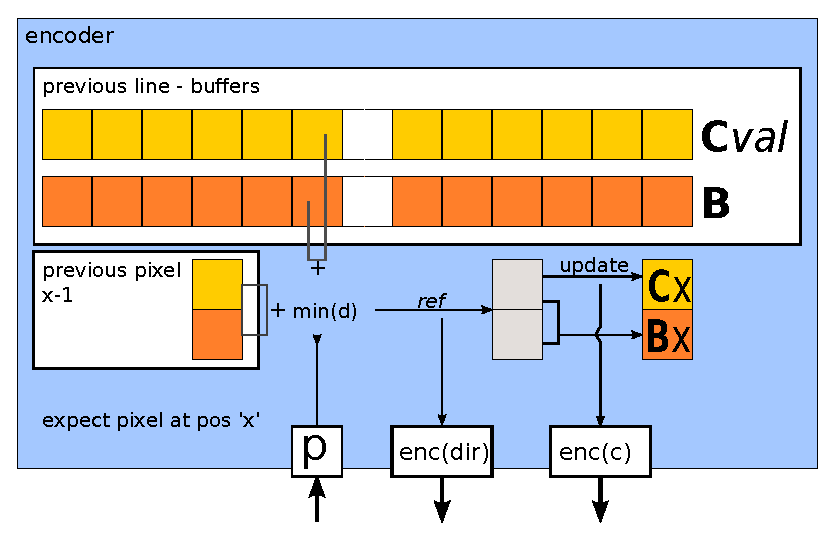
\includegraphics{img/codec-enc2d}
\end{center}
\caption{Schematischer Aufbau eines 2D Encoders}
\label{fig:codec-enc2d}
\end{figure}
%
Die Ausgabewerte $dir$ und $c$ k\"onnen jeweils in einem Bit kodiert werden. Die
Richtung $dir$ als \texttt{0} f\"ur den vertikalen und \texttt{1} f\"ur den
horizontalen Nachbarn. Die Enkodierung $c$ geht bereits aus
Listing~\ref{lst:codec-updt-x} hervor. Ist das Bit gesetzt, wird $c_{va]}$
erh\"oht, andernfalls verringert. In einem Byte k\"onnen so vier Pixel kodiert
werden.
\\
Der Encoder ben\"otigt zus\"atzlich Anweisungen, wann er seinen Zustand f\"ur
das n\"achste Bild bzw. die n\"achste Zeile anpassen muss. Da am linken und oberen
Rand eines Bildes die Vorg\"angerdaten fehlen, werden hier Standardwerte
initialisiert. Im Kompressionsstream werden die Anweisungen \texttt{NEWLINE} 
und \texttt{NEWFRAME} dann als Bit-Muster kodiert. Listing~\ref{lst:cmpr-bit2d} zeigt die 
verwendeten Bit-Muster der 2D Kompression und Tabelle~\ref{tbl:codec-symbols} die 
daraus resultierende \"Ubertragung.

\begin{lstlisting}[caption=Definierte Bit-Muster in der 2D Kompression,%
                   label=lst:cmpr-bit2d]
#define CMPR_ESCAPE     0xFF
#define CMPR_NEW_LINE   0xFE
#define CMPR_NEW_FRAME  0xFD
\end{lstlisting}

\begin{table}[htbp]
\centering
\begin{tabular}{|l|l|}
\hline
Bild-Stream & \"Ubertragung \\ \hline
Anweisung: NEWLINE & CMPR\_ESCAPE CMPR\_NEW\_LINE \\
Anweisung: NEWFRAME & CMPR\_ESCAPE CMPT\_NEW\_FRAME \\
Pixel & C DIR \\
4x (C DIR) = CMPR\_ESCAPE & CMPR\_ESCAPE CMPR\_ESCAPE \\ 
\hline
\end{tabular}
\caption{Kodierung der Anweisungen NewLine und NewFrame}
\label{tbl:codec-symbols}
\end{table}

Ein Bild in der Gr\"osse von 160x120 Pixeln kann so mit etwa $120 \cdot 160/4 + 2 = 5040
\text{bytes}$ kodiert werden.
Die Funktionsweise der Kompression l\"asst bereits erahnen, dass es in Ecken von
horizontalen und vertikalen Kanten zu Artefakten kommen wird. In dieser
Situation gibt es f\"ur den Pixel $p_x$ keine gute Referenz, wodurch sich
$c_{val}$ \"uber einige Iterationsschritte anpassen muss.
Abbildung~\ref{fig:codec2d-artifact} zeigt solche Artefakte anhand unseres
Testvideos. Um diesen Fehler zu minimieren haben wir den Codec im folgenden
Abschnitt um die Referenz zum vorherigen Bild erweitert.
\begin{figure}[tbp]
\begin{center}

\includegraphics[width=0.5\textwidth]{img/codec2d-artifact}
\end{center}
\caption{Artefakte in der 2D Komprimierung}
\label{fig:codec2d-artifact}
\end{figure}
%
%
\section{3D-Komprimierung}
\label{sec:codec3d}
Die Coder der 2D-Komprimierung haben wir so erweitert, dass sie zur
Rekonstruktion auch Bild-Informationen des vorherigen Bildes speichern. Da $b$
und $c_{va]}$ des gesamten Bildes die Speicherkapazit\"at \"uberschreiten
w\"urde, haben wir die Aufl\"osung der Buffer reduziert (Downsampling).
\\
F\"ur die Kodierung $dir$ ergibt sich nun die dritte M\"oglichkeit \textit{last
frame}. Prinzipiell werden f\"ur diese Information zwei Bit ben\"otigt. In
Kombination mit dem \textit{Run-Length-Encoding}, haben wir $dir$ mit einem Bit
kodiert (siehe~\ref{sec:codec-rle}).
\\
Durch Datenverlust kann es passieren, dass der Decoder den Kompressionsstream
nicht weiter verarbeiten kann. Aus diesem Grund haben wir hier eine
Sync-Anweisung eingef\"uhrt, die als \verb@CMPR_FRAME_SYNC 0xFF@ kodiert wird.
Sie bewirkt das Zur\"cksetzen der Buffer auf vordefinierte Standardwerten.
\\
In der Implementierung haben wir die Entwicklung der 3D Coder ohne RLE nicht
weiter verfolgt. Abbildung~\ref{fig:codec3d-artifact} analog zu
Abbildung~\ref{fig:codec2d-artifact} die Kantenartefakte der Kodierung am
Testvideo.
%
\begin{figure}[tbhp]
\begin{center}

\includegraphics[width=0.5\textwidth]{img/codec3d-artifact}
\end{center}
\caption{Reduzierung der Artefakte durch 3D Komprimierung}
\label{fig:codec3d-artifact}
\end{figure}
%
%
%
%
\section{Run-Length-Encoding}
\label{sec:codec-rle}
Gedanke hinter dem Run-Length-Encoding ist es, die Richtung des letzten kodierten
Pixels zu bevorzugen. Wurde der letzte Pixel beispielsweise mit seinem
horizontalen Nachbarn kodiert, erh\"ahlt die horizontale Richtung beim Encoding
des n\"achsten Pixels eine h\"ohere Gewichtung. Ziel ist es \"uber den Verlauf
einer Zeile so wenig \"Anderungen des $dir$ wie m\"oglich zu erzeugen. In der
Konsequenz tritt $dir$ derart wiederholt auf, dass es optimal RLE codiert
werden kann (Abb.~\ref{fig:codec3d-rle}).
\\
\begin{figure}[tbhp]
\begin{center}
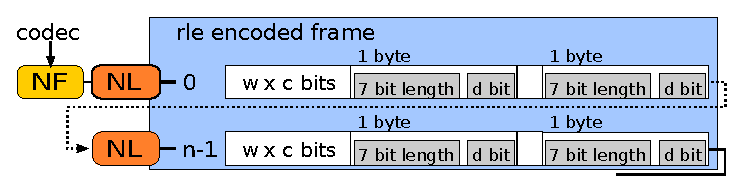
\includegraphics{img/codec3d-rle}
\end{center}
\caption{Kodierung mit Run-Length-Encoding des $d$}
\label{fig:codec3d-rle}
\end{figure}
%
Die Sementik der RLE-Kodierung der Richtung sieht so aus, dass das d-Bit eines
Bytes die \"Anderung der Referenzrichtung nach $n$ Pixeln bewirkt, wobei $n$ in
den verbleibenden sieben Bits gespeichert wird. Auf RLE-Basis komprimierte
Bilder k\"onnen so nur noch zeilenweise dekodiert werden. Wie das d-Bit
verstanden werden kann, beschreibt die Implementierung in 
Listing~\ref{lst:decode-d} in einer Zeile. Die vorherige Richtung muss nat\"urlich
bekannt sein.


\begin{lstlisting}[caption=Dekodierung d-Bits eines RLE-Bytes,%
                   label=lst:decode-d]
/**
 * Decodes change of directon.
 * @parma old   old direction
 * @param flag  direction flag
 * @return      new direction
 *
 * @see cmpr3_encode_dir
 */
static inline int cmpr3_decode_dir(int old, char flag) {
    return flag ? (old == PREVIOUS ? VERTICAL : PREVIOUS) 
                : (old == HORIZONTAL ? VERTICAL : HORIZONTAL);
}
\end{lstlisting}

